\documentclass{article}
\usepackage{graphicx}
\usepackage{listings}
\lstset{language=C}
\graphicspath{ {./images/} }
\usepackage{hyperref}
\hypersetup{
    colorlinks=true,
    linkcolor=blue,
    filecolor=magenta,
    urlcolor=cyan,
}
\lstset{basicstyle=\sffamily}
\usepackage{array}
\usepackage[table]{xcolor}

\begin{document}
\title{Admin Dashboard}

\section{Summary}

Implement a prototype admin dashboard that collects and displays usage metrics submitted
by fake IOT clients.

\section{Rationale}

We would like to evaluate your skills in the following areas:

\begin{itemize} %
  \item Writing design docs.
  \item Writing production quality code for both client and server.
  \item Communicating with the team when working on the challenge.
  \item Handling the feedback received from Teleport engineers.
\end{itemize}

We believe this technique is not only better, but also is more fun compared to whiteboard/quiz interviews so common in the industry. It's not without the downsides - it could take longer than traditional interviews.

\par

\href{https://sockpuppet.org/blog/2015/03/06/the-hiring-post/}{Some of the best teams use coding challenges.}

We appreciate your time and are looking forward to hack on this project together.

\section{Tools}

\begin{center}
\rowcolors{1}{gray!80!gray!50}{gray!50!gray!20}
\begin{tabular}{ | m{15em} | m{15em}| }
  \hline
  Backend & Golang or Rust \\
  \hline
  Frontend & JavaScript or Typescript, pick any framework you like \\
  \hline
  Database & Postgres, MySQL, SQLite \\
  \hline
  Version Control & GitHub \\
  \hline
  Reproducible Builds & Use Docker to package and run your application \\
  \hline
  Code and Tools Provided by us & \href{https://github.com/gravitational/challenge-user-management}{CSS \& HTML}, \href{https://github.com/gravitational/fakeiot}{Fake IOT device emulator and protocol spec} \\
  \hline
  \end{tabular}
\end{center}

\section{Requirements}

  There are 6 engineering levels at Teleport. It's possible to score on level 1-5 through coding challenge.
  Level 6 is only for internal promotions. Check the engineering levels document for more details.

  Start with a very brief google doc that covers the edge cases and design approach and post it to the slack channel. After the doc is approved, implement interfaces and an example program using the library.

  Add a couple of high quality tests that cover happy and unhappy scenarios.

  Split the submission in 2-3 pull requests for us to review. We will review every pull request and provide our feedback.

  We are going to compile the program, test it and get back to you.

  \section{Project Description}

  Implement a server that will be receiving requests from imaginary IOT clients and tracking the number of registered IOT devices.

  You do not need to implement the IOT client. Teleport provides a \href{https://github.com/gravitational/fakeiot}{reference IOT client implementation} to aid you in developing and testing your server.

  The server should have the following functionality:

  Provide the HTTP API compatible with the reference IOT client mentioned above. The reference client can be used to generate data (register fake IOT devices) and test your server. See \href{https://github.com/gravitational/fakeiot}{client} for more information about the API the client expects the server to provide.

Serve the admin dashboard that displays the number of currently registered IOT clients for a particular account. See the mockups for the dashboard UI and interaction flows below. HTML and CSS assets for the dashboard are provided by Teleport: \href{https://github.com/gravitational/challenge-user-management}{user management}

By default the account should be assigned a “Standard Plan” that only allows a certain maximum number of registered IOT devices. The dashboard should provide the ability to upgrade the account to an “Enterprise Plan” once the limit of registered users/devices is reached.


  \subsection*{Level 1}

  \subsubsection*{Login Form}

  Admin signs in on the login page.

  \begin{center}
    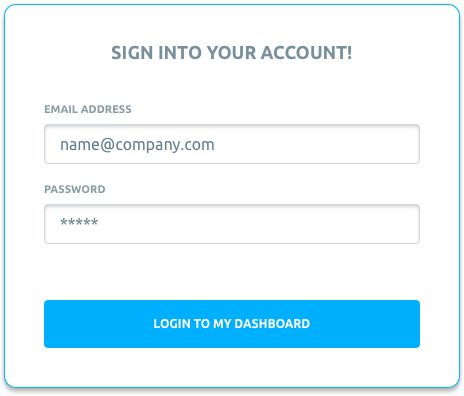
\includegraphics[width=\textwidth]{login}
  \end{center}

  \begin{itemize}
  \item Implement authentication and session management in the most secure way possible.
  \item Do not store the password in plain text. Pick the most secure algorithm of storing password hashes.
  \item Web client should use email and password for authentication.
  \item Server-side form is ok.
  \item Implement logout and session timeout.
  \item Application should not be vulnerable to typical web security vulnerabilities like XSS, CSRF, and SSRF.
  \item Use Makefiles and Docker to allow us to easily build and run your application.
  \end{itemize}

  \subsection*{Level 2}

  \subsubsection{Current Plan}

  Once the admin is logged in, the dashboard displays the current plan and the number of registered/available seats for IOT clients. The progress bar and device count should update periodically without the user refreshing the browser.

  \begin{center}
    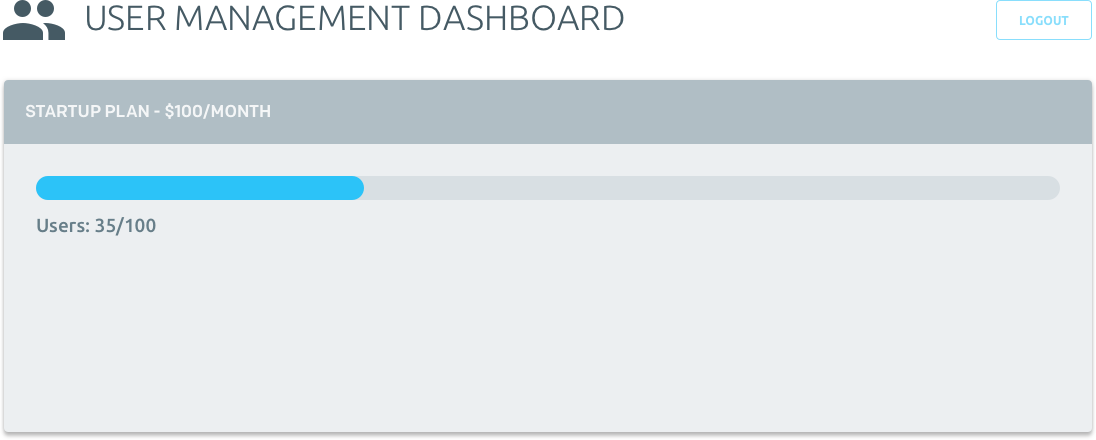
\includegraphics[width=\textwidth]{dashboard-initial}
  \end{center}

  \begin{itemize}
  \item It's OK to use polling for the refresh.
  \item Add HTTPS API with Bearer Token authentication to collect metrics from the client.
     Please Pick Bearer Token key format carefully. There are great and very simple Bearer Token key formats to use, for example, a properly randomized bearer token with sufficient length. The server HTTPS certificate is provided in the fake IOT client repository: \href{https://github.com/gravitational/fakeiot/tree/master/fixtures}{server x509 cert}.
  \end{itemize}

  \subsubsection{Limit Reached}
   Once the account has reached its limit (100/100 seats assigned), the dashboard should prompt the admin to upgrade their account.

  \begin{center}
  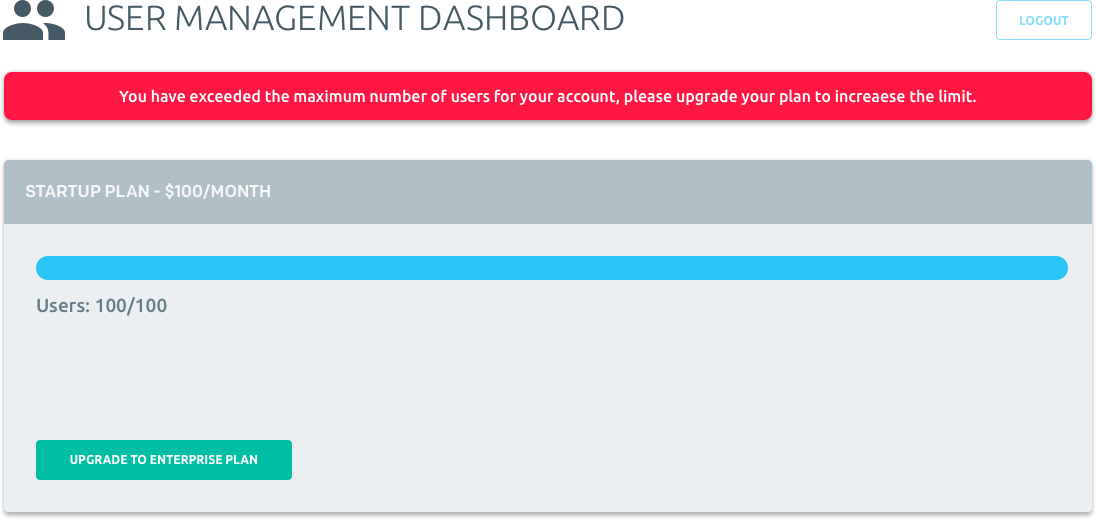
\includegraphics[width=\textwidth]{dashboard-full}
  \end{center}

  \subsubsection{Plan Upgrade}

  Once the plan has been upgraded successfully, the dashboard should display a success message along with the updated plan name and device limits.

  \begin{center}
    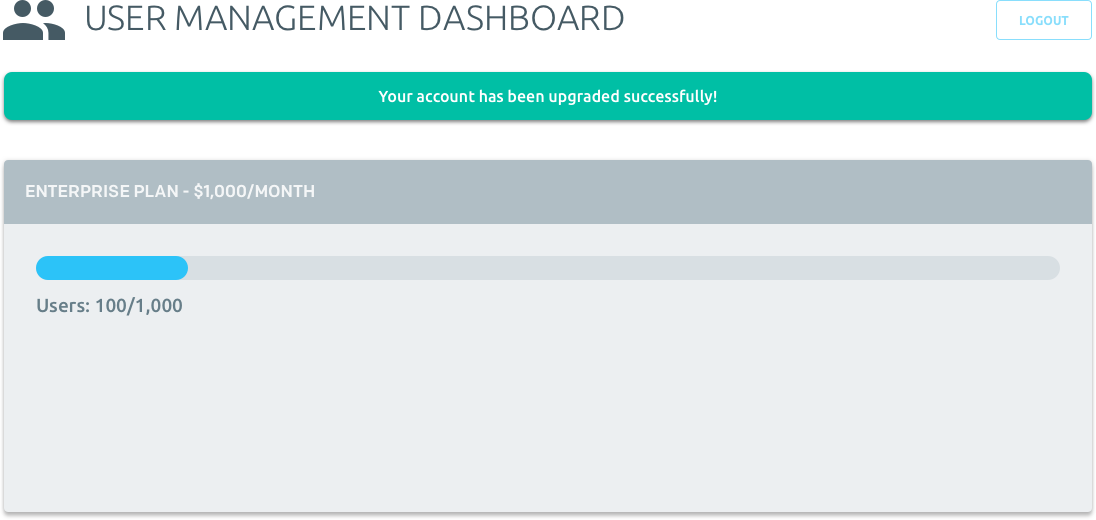
\includegraphics[width=\textwidth]{dashboard-upgraded}
  \end{center}

  \subsection*{Levels 3-4}

  \begin{itemize}
  \item Use realtime event system instead of the polling for metrics update.
  \end{itemize}

\section{Guidance}

\subsection{Interview process}

The interview team joins the slack channel. The team consists of the engineers who will be working with you.
Ask them bout the engineering culture, work and life balance, or anything else that you would like to learn about Teleport.

Before writing the actual code, create a brief design document in Google Docs or markdown in Github and share with the team.

This document should consist of key trade-offs and key design approaches. Please avoid writing overly detailed design document. Use this document to make sure the team could provide feedback on your design and demonstrate that you've investigated the problem space.

Split your code submission using pull requests and give the team an opportunity to review the PRs. A good “rule of thumb” to follow is that the final PR submission is a formality adding a small feature set - it means that the team had an opportunity to contribute the feedback during multiple well defined stages of your work.

Our team will do their best to provide a high quality review of the submitted pull requests in a reasonable time frame. You are spending your time on this, we are going to contribute our time too.

After the final submission, the interview team will assemble and vote using +1, -2 anonymous voting system: +1 is submitted whenever a team member accepts the submission, -2 otherwise.

In case of a positive result, we will connect you to our HR team who will collect one-two references and will work out other details. You can start the reference collection process in parallel if you would like to speed up the process.

After reference collection, our ops team will send you an offer.

In case of a negative score result, hiring manager will contact you and send a list of the key observations from the team that affected the result.

\subsection{Code and project ownership}

This is a test challenge and we have no intent of using the code you've submitted in production.
This is your work, and you are free to do whatever you feel is reasonable with it.
In the scenario when you don't pass, you can open source it with any license and use it as a portfolio project.

\subsection{Areas of focus}

Teleport focuses on networking, infrastructure and security.

These are the areas we will be evaluating in the submission:

  \begin{itemize}
  \item Use consistent coding style. We follow \href{https://github.com/golang/go/wiki/CodeReviewComments}{Golang Coding Style} for the Go language and \href{https://github.com/airbnb/javascript}{AirBnB Coding Style} for the JS language. If you are going to use a different language, please pick coding style guidelines and let us know what they are.
  \item Create one test for unhappy scenario.
  \item Make sure builds are reproducible. Pick any vendoring/packaging system that will allow us to get consistent build results.
  \item Ensure error handling and error reporting is consistent. The system should report clear errors and not crash under non-critical conditions.
  \item Avoid concurrency and networking errors. Most of the issues we've seen in production are related to data races, networking error handling or goroutine leaks. We will be looking for those errors in your code.
  \end{itemize}

\subsection{Trade-offs}

Write as little code as possible, otherwise this task will consume too much time and code quality will suffer.

Please cut corners, for example configuration tends to take a lot of time, and is not important for this task.

Use hard codes as much as possible and simply add TODO items showing your thinking, for example:

\begin{lstlisting}[caption=TODO example]

  // TODO: Add configuration system.
  // Consider using CLI library to support both
  // environment variables and reasonable default values,
  // for example https://github.com/alecthomas/kingpin

\end{lstlisting}

Comments like this one are really helpful to us.
They save yourself a lot of time and demonstrate that you've spent time thinking about this problem and provide a clear path to solution.

Consider making other reasonable trade-offs. Make sure you communicate them to the interview team.

Here are some other trade-offs that will help you to spend less time on the task:

Do not implement a system that scales or is highly performing. Describe which performance improvements would you add in the future?
High availability. It is OK if the system is not highly available. Write down how you would make the system highly available and why your system is not.

\subsubsection*{Testing}

Please don’t overdo the testing. This could take a very long time and distract you from completing the task. Instead, demonstrate your approach for back-end and frontend testing with:

  \begin{itemize}
  \item 1 unit test for the backend.
  \item 1 unit test for the frontend.
  \end{itemize}

The tests should cover both the happy path (function/procedure success) and several error paths (failure due to bad input, failed dependency, etc). Please demonstrate both good test structure and your analysis of edge cases and possible failures.

\subsection{Pitfalls and Gotchas}

  To help you out, we've composed a list of things that previously resulted in a no-pass from the interview team:

    \begin{itemize}
    \item Scope creep. Candidates have tried to implement too much and ran out of time, energy. To avoid this pitfall, use the simplest solution that will work. Avoid writing too much code. We've seen candidate's code introducing caching and making many mistakes in the caching layer validation logic. Not having caching would have solved this problem.
    \item Data races. We will scan the code with a race detector and do our best to find data races in the code. Avoid global state as much as possible, if using global state, write down a good description why it is necessary and protect it against data races.
    \item Deadlocks. When using mutexes, channels or any other synchronization primitives, make sure the system won't deadlock. We've seen candidate's code holding mutex and making a network call without timeouts in place. Be extra careful with networking and sync primitives.
    \item Unstructured code. We've seen candidates leaving commented chunks of code, having one large file with all the code, not having code structure at all.
    \item Not communicating. Candidates who submitted all the code to master branch, which does not give us the ability to provide feedback on the various implementation phases. Because we are a distributed team, structured communication is critical to us.
    \item Implementing custom security algorithms/authentication schemes is always a bad idea unless you are a trained security researcher/engineer. It is definitely a bad idea for this task - try to stick to industry proven security methods as much as possible.
    \end{itemize}

\subsection{Scoring}

We want to be as transparent as possible on how we will be scoring your submission.
The following table provides a description of different areas you will be evaluated on and how they will affect your overall score.

\begin{center}
\rowcolors{2}{gray!80!gray!50}{gray!50!gray!20}
\begin{tabular}{ | m{25em} | m{5em}| m{5em} | }
  \hline
  \rowcolor{blue!60!black!10}
  Description & Points Awarded & Points Subtracted \\
  \hline
  The submitted code has a clear and modular structure & +1 & -1 \\
  \hline
  The candidate communicated their progress during the interview & +1 & -1 \\
  \hline
  The program builds are reproducible & +1 & -1 \\
  \hline
  README provides clear instructions & +1 & -1 \\
  \hline
  The candidate outlined the key design points in the design document & +1 & -1 \\
  \hline
  Client side code is not vulnerable to CSRF and other attacks & +1 & -1 \\
  \hline
  Server side code uses strong HTPS configuration and security & +1 & -1 \\
  \hline
  The code provides examples of tests covering key components & +1 & -1 \\
  \hline
  The code provides clear error handling and reporting & +1 & -1 \\
  \hline
  The program is working according to the specification & +1 & -1 \\
  \hline
  The candidate demonstrates ability to handle and apply feedback & +1 & -1 \\
  \hline
\end{tabular}
\end{center}

\subsection{Questions}

It is OK to ask the interview team questions. Some folks stay away from
asking questions to avoid appearing less experienced, so we provide examples of questions
to ask and questions we expect candidates to figure out on their own.

Here is a great question to ask:

``Is it OK to pre-generate secret data and put the secrets in the repository for the purposes of POC? I will add a note that we will auto-generate secrets in the future.''

It demonstrates that you thought about this problem domain, recognize the trade off and save you and the team time by not implementing it.

This is the question we expect candidates to figure out on their own:

``What version of Go should I use? What dependency manager should I use?''

Unless specified in the requirements, pick the solution that works best for you.

\section{Timing}

It should take you from 4 to 24 full hours to complete the challenge.

You can split coding over a couple of weekdays or weekends and find time to ask questions and receive feedback.

Once you join the slack channel, you have maximum 2 weeks to complete the challenge.

Within this timeframe we are not scoring challenges submitted faster as higher.
We only evaluate quality of the submission.

We only start the coding challenge if there are several open positions available and let
all candidates finish the code submission.


\section{FAQ}

\begin{itemize} %
  \item[] Q: Why can't I use NodeJS for the server side?
  \item[] A: All \href{https://github.com/gravitational/teleport}{Teleport server side code} is implemented in Go.
It's important for us to understand the systems level engineering skills fullstack engineers have.
\end{itemize}

\end{document}
